\documentclass[tikz,border=10pt]{standalone}
\usepackage{pgfplots}
\pgfplotsset{compat=1.17}
\usetikzlibrary{calc, arrows, positioning, shapes.geometric, backgrounds, patterns}
\usepgfplotslibrary{fillbetween, groupplots}
\begin{document}

% Q1
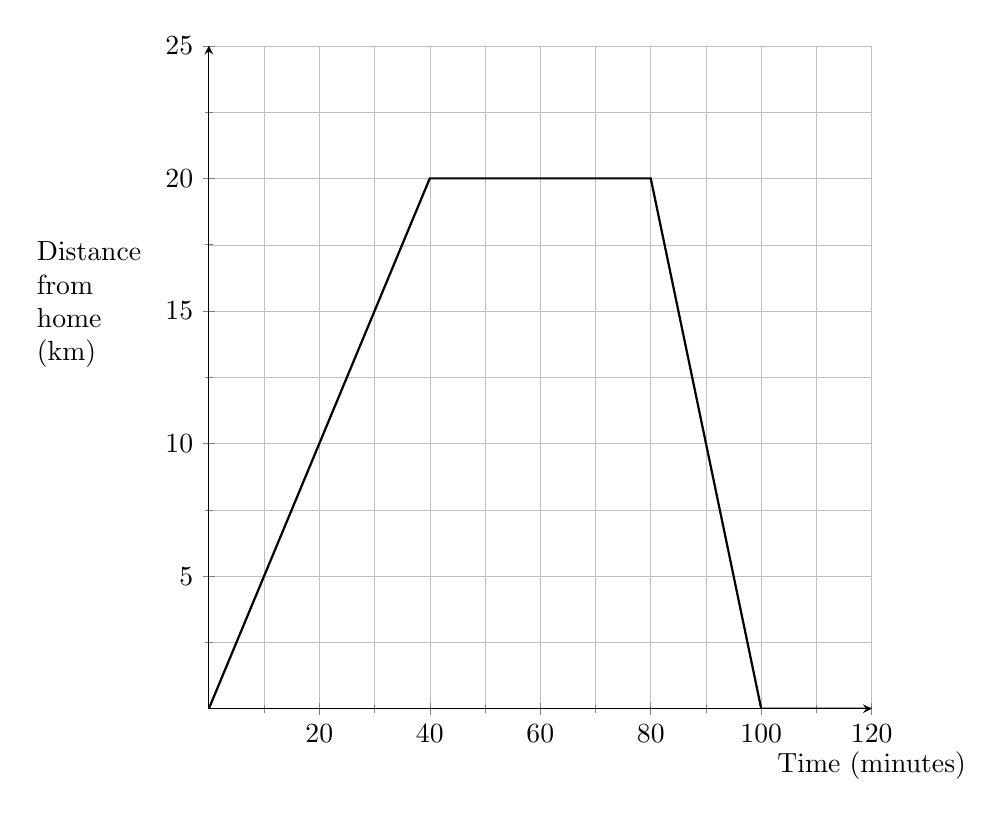
\begin{tikzpicture}
\begin{axis}[
    xlabel={Time (minutes)},
    ylabel={\parbox{1cm}{Distance from home (km)}},
    axis lines=middle,
    grid=both,
    grid style={line width=.1pt, draw=gray!50},
    major grid style={line width=.2pt, draw=gray!50},
    minor tick num=1,
    xmin=0,
    xmax=120,
    ymin=0,
    ymax=25,
    xtick={0,20,40,60,80,100,120},
    ytick={0,5,10,15,20,25},
    xlabel style={at={(axis description cs:1,-0.05)},anchor=north},
    ylabel style={at={(axis description cs:-0.2,0.5)},anchor=south},
    legend pos=outer north east,
    width=10cm,
    height=10cm,
]
\addplot[thick, black] coordinates {(0,0) (40,20) (80,20) (100,0) (120,0)};
\end{axis}
\end{tikzpicture}

% Q2
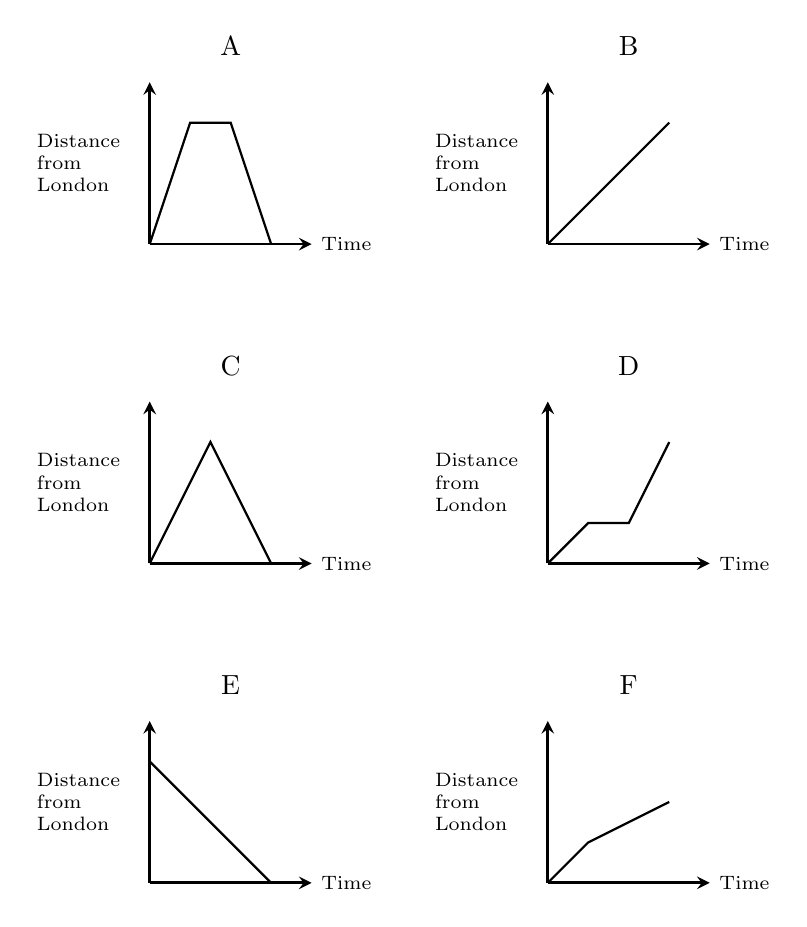
\begin{tikzpicture}
    \begin{groupplot}[
        group style={
            group name=my plots, 
            group size=2 by 3, 
            horizontal sep=3cm, 
            vertical sep=2cm
        },
        width=0.3\textwidth, 
        height=0.3\textwidth,
        axis lines=middle,
        axis line style={line width=1pt},
        xlabel={Time},
        ylabel={\parbox{1cm}{Distance from London}},
        xlabel style={anchor=west, font=\scriptsize},
        ylabel style={at={(axis description cs:-0.15,0.5)},anchor=east, font=\scriptsize},
        xtick=\empty,
        ytick=\empty,
        xmin=0,
        xmax=4,
        ymin=0,
        ymax=4,
        every axis plot/.append style={thick, black}
    ]
        \nextgroupplot[title=A]
            \addplot[no marks] coordinates {(0,0) (1,3) (2,3) (3,0)};
        
        \nextgroupplot[title=B]
            \addplot[no marks] coordinates {(0,0) (3,3)};
        
        \nextgroupplot[title=C]
            \addplot[no marks] coordinates {(0,0) (1.5,3) (3,0)};
        
        \nextgroupplot[title=D]
            \addplot[no marks] coordinates {(0,0) (1,1) (2,1) (3,3)};
        
        \nextgroupplot[title=E]
            \addplot[no marks] coordinates {(0,3) (1,2) (3,0)};
        
        \nextgroupplot[title=F]
            \addplot[no marks] coordinates {(0,0) (1,1) (3,2)};
    \end{groupplot}

\end{tikzpicture}

% Q3
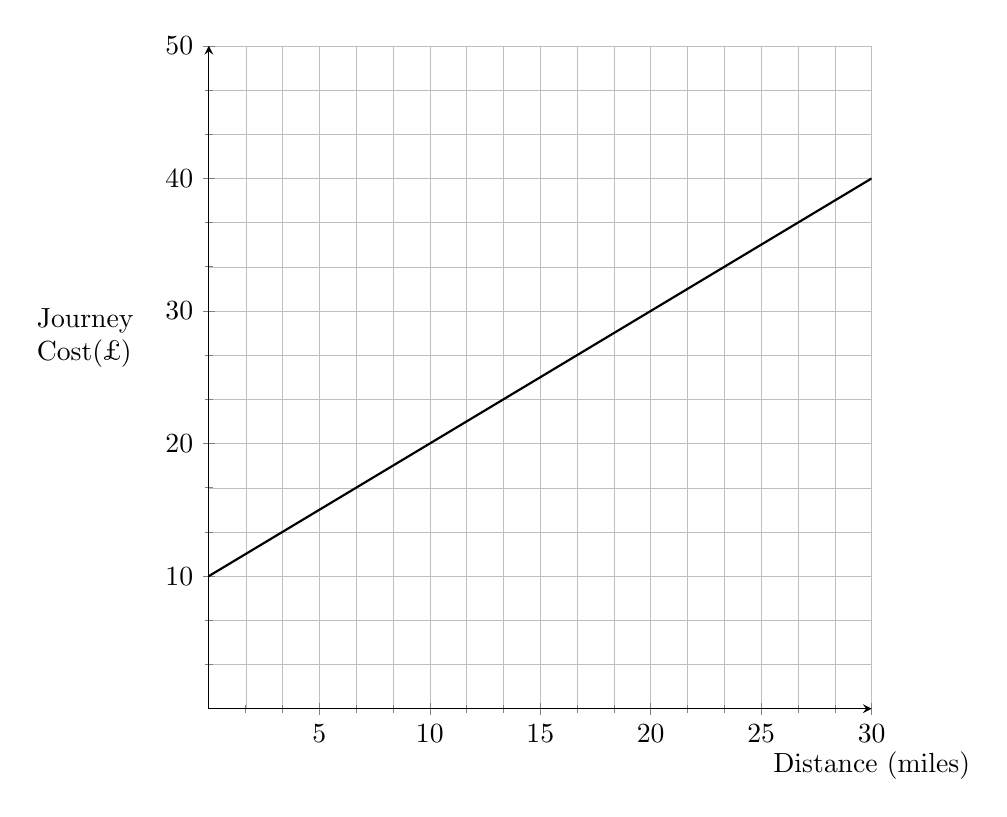
\begin{tikzpicture}
\begin{axis}[
    xlabel={Distance (miles)},
    ylabel={\parbox{1cm}{Journey Cost(£)}},
    axis lines=middle,
    grid=both,
    grid style={line width=.1pt, draw=gray!50},
    major grid style={line width=.2pt, draw=gray!50},
    minor tick num=2,
    xmin=0,
    xmax=30,
    ymin=0,
    ymax=50,
    xtick={0,5,10,15,20,25,30},
    ytick={0,10,20,30,40,50},
    xlabel style={at={(axis description cs:1,-0.05)},anchor=north},
    ylabel style={at={(axis description cs:-0.2,0.5)},anchor=south},
    legend pos=outer north east,
    width=10cm,
    height=10cm,
]
\addplot[thick, black] coordinates {(0,10) (30,40)};
\end{axis}
\end{tikzpicture}

% Q4
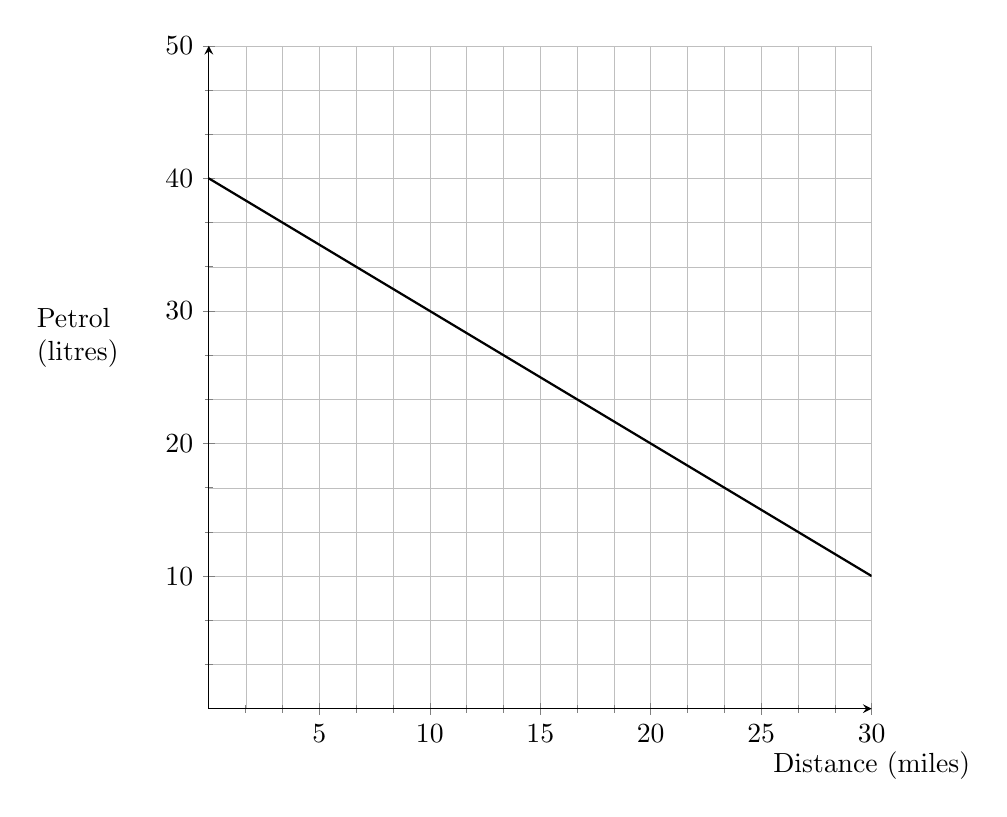
\begin{tikzpicture}
\begin{axis}[
    xlabel={Distance (miles)},
    ylabel={\parbox{1cm}{Petrol (litres)}},
    axis lines=middle,
    grid=both,
    grid style={line width=.1pt, draw=gray!50},
    major grid style={line width=.2pt, draw=gray!50},
    minor tick num=2,
    xmin=0,
    xmax=30,
    ymin=0,
    ymax=50,
    xtick={0,5,10,15,20,25,30},
    ytick={0,10,20,30,40,50},
    xlabel style={at={(axis description cs:1,-0.05)},anchor=north},
    ylabel style={at={(axis description cs:-0.2,0.5)},anchor=south},
    legend pos=outer north east,
    width=10cm,
    height=10cm,
]
\addplot[thick, black] coordinates {(0,40) (30,10)};
\end{axis}
\end{tikzpicture}

% Q5
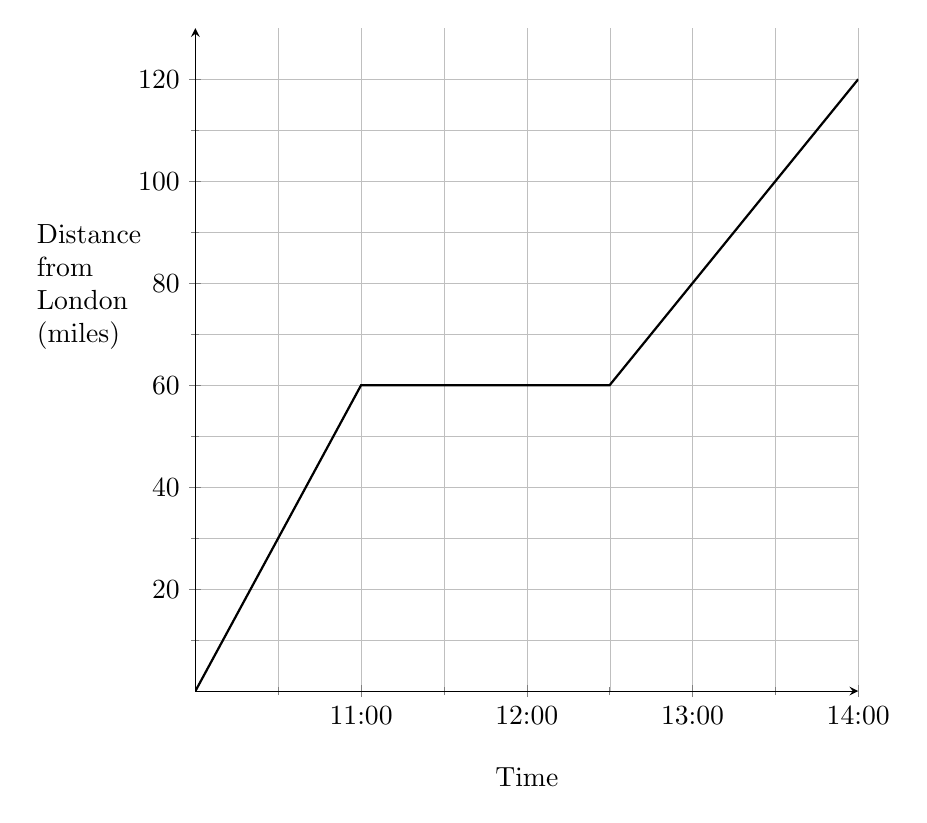
\begin{tikzpicture}
\begin{axis}[
    xlabel={Time},
    ylabel={\parbox{1.5cm}{Distance from London (miles)}},
    axis lines=middle,
    grid=both,
    grid style={line width=.1pt, draw=gray!50},
    major grid style={line width=.2pt, draw=gray!50},
    minor tick num=1,
    xmin=10,
    xmax=14,
    ymin=0,
    ymax=130,
    xtick={10,11,12,13,14},
    xticklabels={10:00, 11:00, 12:00, 13:00, 14:00},
    ytick={0,20,40,60,80,100,120},
    xlabel style={at={(axis description cs:0.5,-0.1)},anchor=north},
    ylabel style={at={(axis description cs:-0.15,0.5)},anchor=south},
    width=10cm,
    height=10cm,
]
\addplot[thick, black] coordinates {(10,0) (11,60) (12.5,60) (14,120)};
\end{axis}
\end{tikzpicture}

\end{document}
